In science, mathematical frameworks are used to study the behavior of objects. In physics, for example, the newton's laws laid the foundation of classical mechanics used to describe the motion of macroscopic objects.
In this thesis, we are interested in the problem of sequential decision making. The most popular mathematical framework used to study sequential decision making is called Markov Decision Process(MDP). The underlying core assumption is the Markovian assumption on the state space. MDP assumes the state space is fully observable and the future is independant of the past conditioned on the current state. More formally, this can be described as:
\begin{equation}
        p(s_{t+1} | s_{t},s_{t-1},...,s_0) = p(s_{t+1} | s_t)
\end{equation}
Sequential decision making differs from supervised learning in several ways. Supervised learning is a set of models designed to predict an output based on IID data. However, in reinforcement learning our prediction/decision often impact the distribution of the data. For example, choosing to do turn right at an intersection will siginificantly change the distribution of future states. 

\section{Markov Decision Process}
We now formally introduce the concept used in Markov Decision Process.
\begin{definition}[Markov Decision Process ~(\cite{puterman2014markov})]
A Markov Decision Process (MDP) is defined as a tuple ($\s,\p,\RE$) where:
\begin{itemize}
    \item $\s$ is a discrete set of states 
    \item $\p : \s \times \A \times \s \mapsto [0,1]$ is a transition function 
    \item  $\RE : \s \times \A \mapsto \R$ is a reward function
\end{itemize}
\end{definition}
On each round $t$, the learner observes current state $s_t\in\s$ and selects action $a_t\in\A$, after which it receives reward $r_t = \RE(s_t,a_t)$ and moves to new state $s_{t+1}\sim \p(\cdot|s_t, a_t)$. We define a stationary policy $\pol$ as a probability distribution over actions conditioned on states $\pol : \s \times \A \mapsto [0,1]$, such that $a_t \sim \pol(\cdot|s_t)$.

\section{Policy Evaluation}
For policy evaluation,  given a policy $\pol$, the goal is to find the associated value function of that policy $v^{\pol}$. 
When performing policy evaluation in the discounted case, the goal is to estimate the discounted expected return of policy $\pol$ at a state $s\in\s$,  $\V^{\pol}(s) = \expect_{\pol}[\sum_{t=0}^{\infty} \gamma^t \RE_{t+1} | s_0 = s]$, with discount factor $\gamma \in [0,1)$. This can be written in matrix form as:
\begin{equation}
     v^{\pol} = \sum_{i=0}^{\infty} \gamma^i (P^{\pol})^i r
\end{equation}
where $P^{\pol}$ denotes the $|\s|\times |\s|$ transition matrix under policy $\pol$, $v^\pi$ is the state values column-vector, and $r$ is the reward column-vector. The actions do not appear in the equations explicitly as the policy has been coupled inside $P^{\pol}$.The matrix $P^{\pol}$ also defines a Markov chain.
In practice, we often do not have  access to the transitions and rewards directly. Instead, we sample tuples $(s,s',r)$ from the environment and use those to estimate in expectation the discounted expected cumulative return for a state.
The most straightforwad way to estimate $v$ would be to collect tuples $(s,s',r)$  and average the discounted reward. However, this often suffers from high variance (\cite{kearns2000bias}). By unrolling the discounted sum of reward it is possible to obtain a recursive form based on $v$:
\begin{equation}
\label{equ:bellman}
\begin{split}
    v^{\pol}(s_0) &=  \expect_{\pol}[\RE (s_0,\pol(s_0)) + \sum_{t=1}^{\infty} \gamma^t \RE_{t+1} | s_0 = s] \\
    &=  \expect_{\pol}[\RE (s_0,\pol(s_0)) + \gamma \expect_{\pol}[\sum_{t=0}^{\infty} \gamma^t \RE_{t+1}|s_1] | s_0 = s]\\
    &= \expect_{\pol}[\RE (s_0,\pol(s_0)) + \gamma v^{\pol}(s_1) | s_0 = s] \\
\end{split}
\end{equation}
This can also be rewritten as a linear system of equation and solved using standard algebra methods:
\begin{equation}
\label{eq:fixed_point}
\begin{split}
    & v^{\pol} = r + \gamma P^{\pol}v^{\pol} \\
    &\equiv (I-P^{\pol})v^{\pol} = r
\end{split}
\end{equation}
However, inverting a matrix can be costly, unstable and as mentioned earlier in practice we often do not have access to $P^{\pol},r$ directly. This suggests that using iterative method may be more suitable for reinforcement learning.
\subsection{Bellman Operator}
We consider the operator-theoretic point of view by defining the following operator
\begin{definition}
The Bellman operator $\T^{\pol}$ has a unique fixed point $v^{\pol}$  where:
\begin{equation}
\label{equ:bell_pol}
   \T^{\pol} v = r + \gamma P^{\pol} v
\end{equation}
\end{definition}
In order to show this we use Banach Fixed point theorem stating that:
\begin{theorem}[Banach Fixed Point Theorem (\cite{banach1922operations})]
Let U be a Banach space: if $\T U \rightarrow U$ is a contraction mapping then:
\begin{itemize}
    \item There exists a unique fixed point $v^*$ such that $\T v^* = v^*$
    \item $lim_{t \rightarrow \infty} \T^tv = v^*$ 
\end{itemize}
\end{theorem}

As we saw in the previous section in equation \ref{eq:fixed_point} $v^{\pol}$ is a fixed point. We can prove its unicity and the convergence of the operator by proving that $ \T^{\pol}$ is a contraction. In this thesis, unless stated otherwise, the norm considered is the infinity norm.
\begin{lemma}
$\T^{\pol}$ is a contraction with a contraction factor of $\gamma$
\end{lemma}
\begin{proof}
\begin{equation}
\begin{split}
    \norm{\T^{\pol}u - \T^{\pol} v} &= \norm{r+\gamma P^{\pol}u - (r + \gamma P^{\pol} v} \\
    &= \norm{\gamma P^{\pol}(u - v)}\\
    &= \gamma \norm{u-v}
\end{split}
\end{equation}
\end{proof}
Algorithm \ref{alg:pol_eval} shows an example of a stochastic version of equation \ref{equ:bell_pol}.\\

\begin{algorithm}[H]
\caption{Policy evaluation}
\begin{algorithmic}[1]
    \STATE Input: $\pi,\gamma$
    \FORALL{steps}
        \STATE Choose $a \sim \pi(\s)$
        \STATE Take action $a$, observe $r(s),s'$
        \STATE $\V(s) =  r(s) + \gamma \V(s') $
    \ENDFOR
\end{algorithmic}
\label{alg:pol_eval}
\end{algorithm}
It is also possible to study the stochastic version of this operator using techniques from dynamical system and ordinary differential equations (\cite{borkar2000ode}).


\subsection{Temporal Difference}
At each step of the bellman operator the previous estimate $v^{\pol}_t$ at time step t is forgotten.
\begin{equation}
    v_{t+1} = r + \gamma P v_{t}
\end{equation}
Temporal difference attempts to exploit previous estimates by averaging them such that $v_{t+1} = \alpha \sum_{i=0}^{t+1} (1-\alpha)^{t-i} v_i$
\begin{equation}
\begin{split}
    v_{t+1} &= \alpha  (r + \gamma P v_{t}) + (1-\alpha) v_{t} \\
    &= \alpha  (r + \gamma P v_{t}) + (1-\alpha) [\alpha (r + \gamma P v_{t-1}) + (1-\alpha) v_{t-1}]
\end{split}
\end{equation}
This gives rise to the temporal difference algorithm:
\begin{equation}
\begin{split}
    v_{t+1} &= \alpha  (r + \gamma P v_{t}) + (1-\alpha) v_{t} \\
    &= \alpha (r + \gamma P v_{t} - v_{t}) + v_{t}
\end{split}
\end{equation}
\begin{definition}[Temporal Difference ~(\cite{sutton1988learning})]
The temporal difference operator $\T_{\alpha}$ parametrized by $\alpha$ can be written as:
\begin{equation}
\begin{split}
    \T_{\alpha} v &= (1-\alpha)v + \alpha(r + \gamma Pv) \\
\end{split}
\end{equation}
\end{definition}

A stochastic version of temporal difference can be found in algorithm \ref{alg:temporal_difference}.\\
\begin{algorithm}[H]
\caption{Temporal Difference}
\begin{algorithmic}[1]
    \STATE Input: $\pi,\alpha,\gamma$
    \FORALL{steps}
        \STATE Choose $a \sim \pi(\s)$
        \STATE Take action $a$, observe $r(s),s'$
        \STATE $\V(s) = \V(s) + \alpha (r(s) + \gamma \V(s')-\V(s)) $
    \ENDFOR
\end{algorithmic}
\label{alg:temporal_difference}
\end{algorithm}

Bootstrapping on previous estimates may introduce bias depending on how well $v$ is estimated. Several papers attempt to characterize this bias in various ways (\cite{kearns2000bias,sutton1994step}). Methods bootstrapping on previous estimates are also called semi-iterative methods (\cite{varga2009matrix}) in the field of iterative methods. It would be interesting to examine algorithms like chebyshev semi-iterative method (\cite{golub1961chebyshev}) that attempts to find optimal $\alpha$'s using chebyshev polynomials. There might exists interesting connections with meta-learning algorithms.
\subsection{Lambda Return}
In the previous sections we defined algorithms that bootstrap on the next value, to reduce variance, instead of looking at the rewards. Lambda return (\cite{sutton1984temporal}) generalizes this intuition by bootstrapping on all future values, not just the direct next one. This is done by first unrolling the bellman updates, yielding N-step return of the form:
\begin{definition}[N-step return]
\begin{equation}
    \T_{n} = \sum_{i=0}^{n} \gamma^i r + \gamma^{n+1} Pv
\end{equation}
\end{definition}
Instead of choosing a specific N, lambda-return exponentially averages through all the N-step return.
\begin{definition}[Lambda-return]
\begin{equation}
    \T^{(\lambda)} = (1-\lambda) \sum_{i=0}^{\infty} \lambda^i \T_{i}
\end{equation}
\end{definition}

Varying $\lambda$ yields Monte Carlo on one side ($\lambda \rightarrow 1$) and TD(0) on the other ($\lambda \rightarrow 0$).
Lambda-return can be implemented efficiently in an online fashion using eligibility traces (\cite{sutton1984temporal,singh1996reinforcement,precup2000eligibility}).\\
\begin{algorithm}[H]
\caption{Temporal Difference with eligibility traces}
\begin{algorithmic}[1]
    \STATE Input: $\pi,\alpha,\gamma,\lambda$
    \FORALL{steps}
        \STATE Choose $a \sim \pi(\s)$
        \STATE Take action $a$, observe $r(s),s'$
        \STATE $e(t) =  \mathbb{1}_{s}+ \gamma \lambda e(t-1)$
        \STATE $\V = \V + \alpha (r(s) + \gamma \V(s')-\V(s)) e(t)$
    \ENDFOR
\end{algorithmic}
\label{alg:eligibility_traces}
\end{algorithm}
However, this algorithm is biased if the trace is used online. This is due to the fact that when an update is done, the trace becomes biased as the distribution with respect to the new parameters would have been different. True online TD (\cite{seijen2014true}) solves this issue by accounting for those changes. This problem is similar to the one encountered by real time recurrent learning (\cite{williams1995gradient}). It would be interesting to study if True Online TD can be extended to the non-linear settings. 
\subsection{Linear Function Approximation}
The methods developed previously scale linearly with the number of states. This becomes quickly intractable for large discrete state space and continuous settings. One way to remedy this is to use function approximation. It is possible to develop similar operators using function approximator.
The aim is to find a function $V_\theta: \mathbb{S} \rightarrow \mathbb{R}$ parametrized by $\theta$ that approximates $V^{\pol}$. We can fall back to the tabular setting by representing the states in a one hot vector form with $\theta \in \mathbb{R^{|\mathbb{S}|}}$. The goal is to find a set of parameters $\theta$ that minimizes the squared loss:
\begin{equation}\label{simple_loss}
    \mathcal{L}(\theta) = \expect_{\pol} [(V^{\pol} - V_\theta)^2]
\end{equation}
which yields the following update by taking the derivative with respect to $\theta$:
\begin{equation}
    \theta_{t+1} = \theta_t + \alpha (V^{\pol}(s_t) - V_{\theta_t}(s_t)) \nabla_{\theta_t} \Vt(s_t)
\end{equation}
where $\alpha$ is a learning rate.\\
In practice $V^{\pol}$ is approximated using Monte Carlo rollouts (\cite{suttonreinforcement}) or TD methods (\cite{sutton1988learning}).

\subsection{Convergence using Stochastic Approximation}
Convergence in the stochastic setting is usually proven by casting the learning algorithm as a stochastic approximation (\cite{tsitsiklis1994asynchronous,borkar2009stochastic,borkar2000ode}) of the form:
\begin{equation}\label{stoch}
    \theta_{t+1} = \theta_t + \alpha( \T \theta_t  - \theta_t + w(t)) 
\end{equation}
where $\T: \mathbb{R^{|\mathbb{S}|}} \rightarrow \mathbb{R^{|\mathbb{S}|}}$ is a contraction operator and $w(t)$ is a noise term. 
As an example, TD(0) is known to converge to the fixed point of the bellman operator (\cite{sutton1988learning}):
\begin{equation}
\begin{split}
    \T \Vt(s_t) &= \expect_{s_{t+1} \sim \pol} [r(s_t) + \gamma \Vt(s_{t+1})]\\
\end{split}
\end{equation}
However, in practice we have access to a noisy version of the operator $\widetilde{\T}$ due to sampling process hence the noise term $w(t)$:
\begin{equation}
    w(t) = r_t + \gamma \Vt (s_{t+1}) - \expect_{s_{t+1} \sim \pol} [r + \gamma \Vt(s_{t+1})]
\end{equation}

\section{Control}
In the previous section we discussed estimating the value of a policy. However, in many cases, the actual goal is to use this estimate to \emph{improve} on the policy. This is called control.
\subsection{Bellman Optimilatiy Equations}
In the control case, the goal is to find the optimal policy $\pol^*$ that maximizes the discounted expected return. As in the previous section we define the optimal value function $\V^*$ as the fixed point of the non-linear optimal Bellman operator:
\begin{equation}
\label{eq:non_linear}
    \T^* v^* = \max_{a \in \A} [r(a) + \gamma P(a)v^*].
\end{equation}

\subsection{Policy Iteration}
Using the operator defined in eq \ref{eq:non_linear}, we now define our first control algorithm. The main framework used for control in Reinforcement Learning is called Generalized Policy Improvements(GPI) (\cite{sutton1998reinforcement}). GPI alternates between policy evaluation and policy improvements.\\

\begin{algorithm}[H]
\caption{General Policy Improvements}
\begin{algorithmic}[1]
    \STATE Input: $\pi,\alpha,\gamma$
    \STATE Policy Evaluation:
    \begin{ALC@g}
        \FORALL{steps}
            \STATE Choose $a \sim \pi(\s)$
            \STATE Take action $a$, observe $r(s),s'$
            \STATE $\V(s) =  r(s) + \gamma \V(s') $
        \ENDFOR
    \end{ALC@g}
    \STATE Policy Improvement:
    \begin{ALC@g}
        \FORALL{$s \in \s$}
            \STATE $\pi(s) \leftarrow \text{argmax}_a \sum_{s'} p(s',r|s,a) + [r+\gamma \V(s')]$
        \ENDFOR
    \end{ALC@g}
    \STATE If policy stable stop, else go to Policy Evaluation
\end{algorithmic}
\label{alg:GPI}
\end{algorithm}

However, this algorithm requires to have a model of the environment to select the next optimal action. To remedy the concept of Q-function was introduced (\cite{watkins1992q}).

\subsection{Q function}
Q-function are state action pair representing the expected discounted return from $s_0$ if action $a_0$ is to be taken.
\begin{equation}
\begin{split}
    Q(s,a) &= \expect_{\pol}[\sum_{t=0}^{\infty} \gamma^t \RE_{t+1} | s = s_0,a = a_0] \\ 
    &= \expect_{s'}[r_t + \gamma v(s')]\\
    &= \expect_{s'}[r_t + \gamma \text{max}_{a'} Q(s',a')]
\end{split}
\end{equation}
Selecting the optimal action can easily be done by taking the max Q-values over all actions. This algorithm is called Sarsa(State–action–reward–state–action).\\
\begin{algorithm}[H]
\caption{SARSA}
\begin{algorithmic}[1]
    \STATE Input: $\pi,\alpha,\gamma$
    \FORALL{steps}
        \STATE Choose $a \sim \pi(\s)$
        \STATE Take action $a$, observe $r(s),s'$
        \STATE $\Q(s,a) = \Q(s,a) + \alpha(  r(s) + \gamma \Q(s',a') - \Q(s,a)) $
    \ENDFOR
\end{algorithmic}
\label{alg:SARSA}
\end{algorithm}


Estimating the optimal action requires calculating the value of each action and taking the argmax. This can be problematic in continous action space.


\subsection{Policy Gradient}
If the action space is continuous or large, using look-up tables for Q-values can become quickly intractable. One way to circumvent this problem is to use function approximation on the policy. We define a policy $\pol_{\theta}$ parametrized by theta. The goal is to find a set of parameters $\theta$ such as to maximize: $J(\theta)=\expect_{\pol}[\sum_{t=0}^{\infty} \gamma^t \RE_{t+1}]$. 
\begin{definition}[Policy Gradient (\cite{sutton2000policy})]
The gradient $\nabla J(\theta)$ can be expressed as:
\begin{equation}
    \nabla J(\theta) = \int_s d^{\pol}(s) \int_a \nabla_{\theta} \pol(a,s)\Q^{\pol}(s,a)
\end{equation}
\end{definition}
In practice, those integrals can be estimated using samples. Furthermore $\Q$ is often unknown, but can be estimated using rollouts $G_t$ to approximate $\V(s)$. This algorithm is called REINFORCE (\cite{williams1995gradient}).

\subsection{Actor-Critic}
Policy gradient methods can be enhanced by bootstrapping on a learned value function to approximate $G_t$ instead of using Monte Carlo rollouts. This is the central idea behind actor-critic (\cite{konda2000actor}) method which can be summarized in figure \ref{fig:actor_critic}. Actor critic can be thought of as combining policy gradient and value based method. Many of the recent algorithms developed are based on this framework (\cite{mnih2016asynchronous,schulman2017proximal,wu2017scalable}).
\begin{figure}
    \centering
    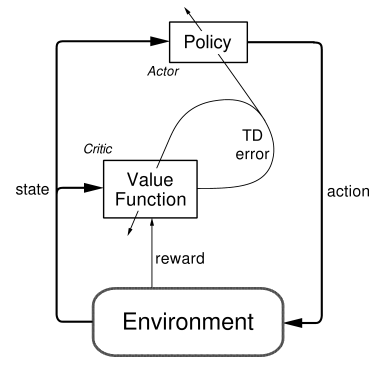
\includegraphics[scale=0.6]{fig/actor_critic.png}
    \caption{Actor-critic}
    \label{fig:actor_critic}
\end{figure}
\section{Deep Reinforcement Learning}
Reinforcement learning algorithms combined with deep neural network as function approximation yields promising results on high dimensional problem (\cite{mnih2013playing,mnih2016asynchronous,schulman2017proximal}) such as Atari (\cite{bellemare2013arcade}) and Mujoco (\cite{todorov2012mujoco}). However, they appear to be very unstable and requires a number of \emph{tricks} to behave properly. We will describe 2 different algorithm Asynchronous Actor Critic ( A3C ~\cite{mnih2016asynchronous}) and Proximal Policy Optimzation (PPO ~\cite{schulman2017proximal}) and explain the tools used to make them stable. Both methods are based on actor critic formulation. 
\subsection{A3C}
One severe problem when using deep neural network as function approximation arise from the fact that the data is not IID. A3C (\cite{mnih2016asynchronous}) is an actor-critic method developed to overcome this issue when used with deep neural networks. This is effectively done by running several agents in parallel and using a batch of data to update the parameters. This effectively decorrelates the samples seen by the agents. A diagram explaining the algorithm can be found in figure \ref{fig:a3c}.
\begin{figure}
    \centering
    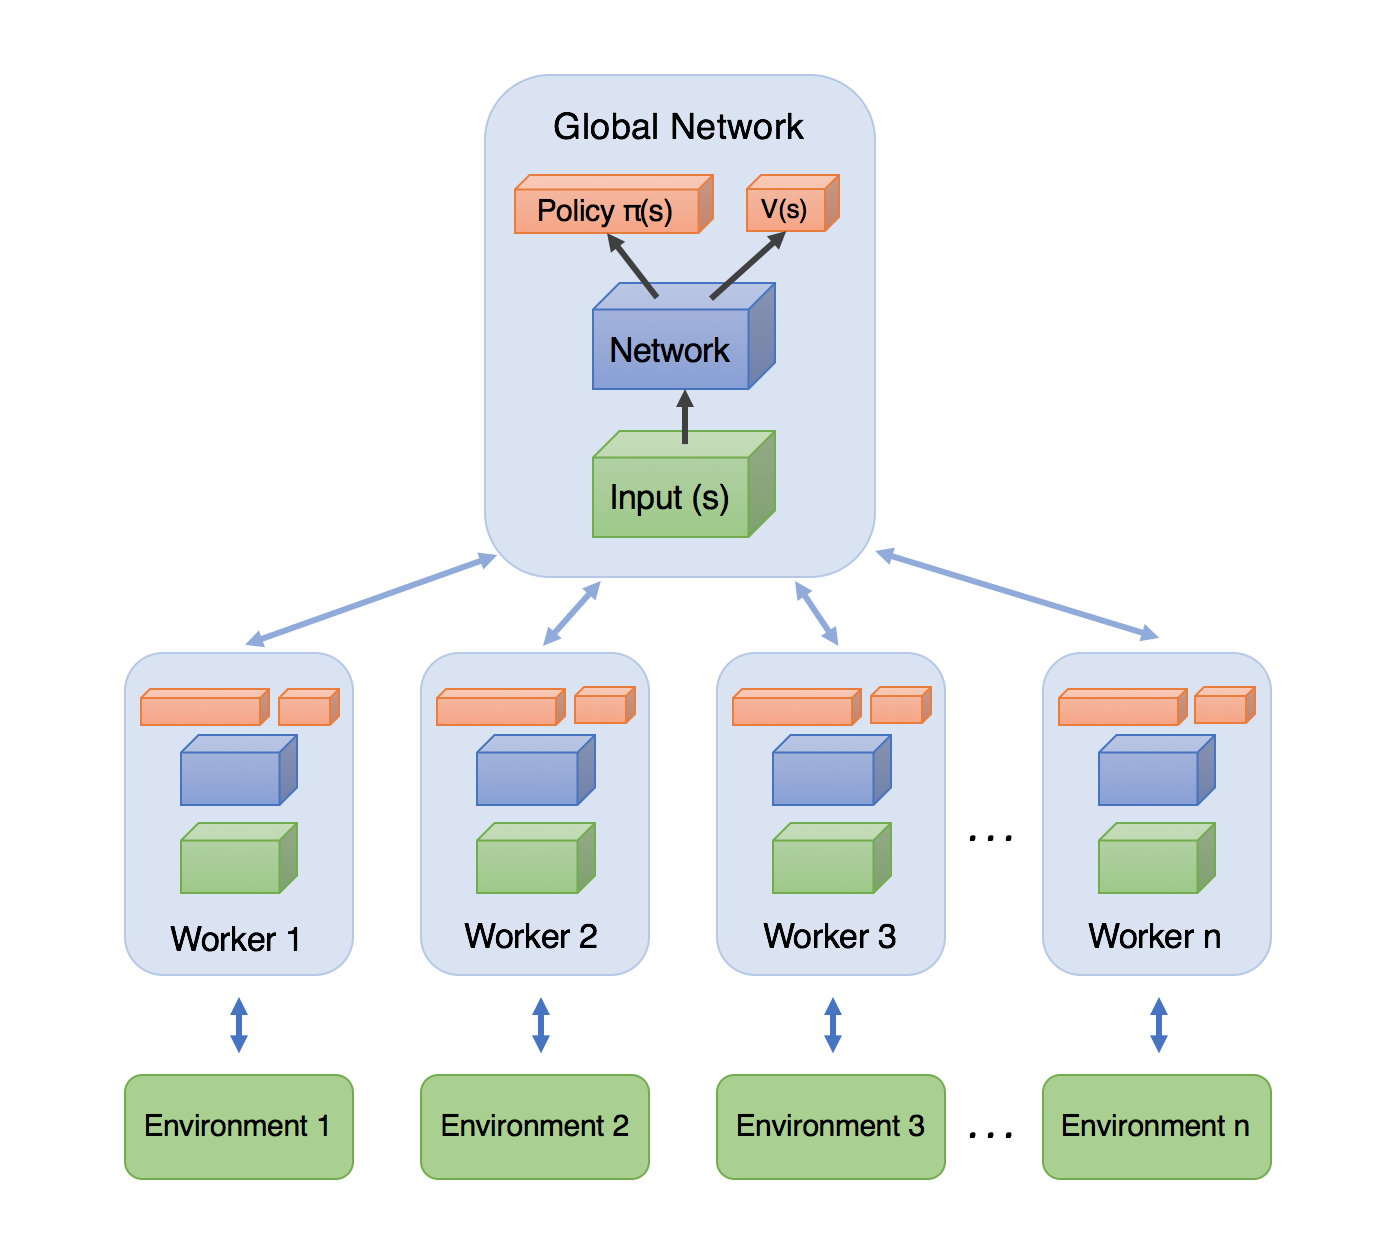
\includegraphics[scale=0.25]{fig/A3C.png}
    \caption{A3C diagram from LOOK AT COPYRIGHT }
    \label{fig:a3c}
\end{figure}
\subsection{PPO}
Another important issue in Reinforcement Learning is the one of non-stationarity of the data.
Proximal methods (\cite{schulman2017proximal,schulman2015trust}) alleviate this by limiting the update of the actor at each time step:
\begin{equation}
    \beta \text{KL}(\pi_{\text{old}},\pol_{\text{new}})
\end{equation}
where $\param$ control the magnitude of the regularization. This regularization has been found to be effective when combined with deep neural network as function approximator.



Regularization in Machine Learning is a cornerstone. Most models can be seen as bias/variance trade-off.
\section{Regularization}
Regularization in RL has been considered in several different perspectives. In this section we discuss the most popular one. Other works focus on regularizing the changes in policy directly. Those approaches are often based on entropy methods (\cite{neu2017unified,schulman2017proximal,bartlett2009regal}).
Explicit regularization in the temporal space has received much less attention.
% Though it has been shown that exploiting \emph{temporal coherence} can benefit to tracking algorithms and thus help in meta-learning~\cite{sutton2007role}, this remains far from the setting considered in this work.
Temporal regularization in some sense may be seen as a ``backward'' multi-step method (\cite{sutton1998reinforcement}). 
\subsection{Spatial Regularization}
 One line of investigation focuses on regularizing the features learned on the state space (\cite{massoud2009regularized,petrik2010feature,pazis2011non,farahmand2011regularization,liu2012regularized,harrigan2016deep}). These approaches assume that nearby states in the state space have similar value.


\subsubsection{Regularization of the function approximation}
\cite{farahmand2011regularization}
This thesis studies the reinforcement learning and planning problems that are modeled by a discounted Markov Decision Process (MDP) with a large state space and finite action space. We follow the value-based approach in which a function approximator is used to estimate the optimal value function. The choice of function approximator, however, is nontrivial, as it depends on both the number of data samples and the MDP itself. The goal of this work is to introduce flexible and statistically-efficient algorithms that find close to optimal policies for these problems without much prior information about them. The recurring theme of this thesis is the application of the regularization technique to design value function estimators that choose their estimates from rich function spaces. We introduce regularization-based Approximate Value/Policy Iteration algorithms, analyze their statistical properties, and provide upper bounds on the performance loss of the resulted policy compared to the optimal one. The error bounds show the dependence of the performance loss on the number of samples, the capacity of the function space to which the estimated value function belongs, and some intrinsic properties of the MDP itself. Remarkably, the dependence on the number of samples in the task of policy evaluation is minimax optimal. We also address the problem of automatic parameter-tuning of reinforcement learning/planning algorithms and introduce a complexity regularization-based model selection algorithm. We prove that the algorithm enjoys an oracle-like property and it may be used to achieve adaptivity: the performance is almost as good as the performance of the unknown best parameters. Our two other contributions are used to analyze the aforementioned algorithms. First, we analyze the rate of convergence of the estimation error in regularized least-squares regression when the data is exponentially beta-mixing. We prove that up to a logarithmic factor, the convergence rate is the same as the optimal minimax rate available for the i.i.d. case. Second, we attend to the question of how the errors at each iteration of the approximate policy/value iteration influence the quality of the resulting policy. We provide results that highlight some new aspects of these algorithms.

\subsection{Policy Regularization}
There exists several ways to regularize policy gradient method. The most comonly used in recent research is called entropy regularization \cite{neu2017unified,schulman2017proximal,bartlett2009regal}.
\subsubsection{Entropy Regularization}
In policy gradient method, one successful approach consists of regularizing the entropy of your policy distribution \cite{neu2017unified}. Policy gradient methods will tend to converge to distributions with low entropy. By adding an entropy bonus, it encourages the policy to explore and often yields much better performance.
\begin{equation}
\begin{split}
    \pol &= \expect_{\pol}{r} + R(\pol)\\
    R(\pol) = \text{entrop}
\end{split}
\end{equation}
This sets of work \cite{schulman2017proximal,schulman2015trust} considers limiting the update of the policy gradient at each step to guarantee \emph{coherent} behavior. 


\subsection{Temporal Regularization}
Though no work explicitely considers the bias and variance induced of considering the past estimates, several work attempts to exploit this relationship to better performance.
\subsubsection{Natural value approximator}
The closest work to ours is possibly \cite{xu2017natural}, where they define natural value approximator by projecting the previous states estimates by adjusting for the reward and $\gamma$. Their formulation, while sharing similarity in motivation, yields different theory and algorithm in practice.
\subsubsection{Backward bootstrapping}
Backward bootstrapping method's can be seen as regularizing in feature space based on temporal proximity \cite{sutton2009fast,li2008worst,baird1995residual}
\subsection{Deliberation cost}
There exists between temporal regularization and option. Indeed having a high deliberation cost \cite{harb2017waiting} means that you smooth out your problem by having longer action. This can be seen as a bias variance trade off. 
\subsubsection{Temporal coherence}
Though it has been shown that exploiting \emph{temporal coherence} can benefit to tracking algorithms and thus help in meta-learning~\cite{sutton2007role}, this remains far from the setting considered in this work.


